\chapter{Inclusion d'éléments exterieurs}\label{chapter:inclus}
	Trois type différent peuvent être inclus dans le livre: les personnages, les items ainsi que les compétences. Chaque types sont ajoutable, modifiable et supprimable grâce à un clique droit dans l'un de ces trois tableaux.
	L'ID de chaque types lui est propre et donc, ne peux subsister qu'un seul id unique par types: un ID de personnage peut être le même qu'un ID de compétences mais ne peut pas être le même qu'un autre ID de personnage.

	\section{Les personnages}
		Un personnage peut être créer en renseignant des champs dans sa boite de dialog. Il ne peut contenir l'id "main\_character", qui lui, est l'id du personnage principal. Mais son nom peut être le même qu'un autre personnage existant.
		Concernant la coche "Double dégâts", elle est la même qu'au personnage principal et permet donc au personnage créer, d'avoir 2 chances sur 5 d'effectuer un double dommage lors de l'attaque dans les noeud de combat (Voir \ref{subsubsection:combat}).
	\begin{figure}[H]
		\centering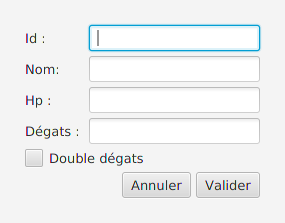
\includegraphics[width=4cm]{img/inclusPersonnages.png}
	\end{figure}

	\section{Les items}
		Des items de toutes sortent peuvent être ajouté: des items de soins, d'attaque, de défense, d'argent et d'autre items basique (par exemple, une clé).
		\begin{itemize}
			\item \textbf{Potion}: peut ajouter de la vie comme en retiré; contient des points d'usures de matériel permettant de savoir combien de fois le joueur peut l'utiliser.
			\item \textbf{Arme}: points d'attaque de l'arme; contient des points d'usures de matériel permettant de savoir combien de fois le joueur peut l'utiliser.
			\item \textbf{Défense}: points de résistance de l'item de défense; contient des points d'usures de matériel permettant de savoir combien de fois le joueur peut l'utiliser.\\
		\end{itemize}

		Ce items peuvent être acheter ou pris dans le prélude ou acheter/pris/utiliser dans les noeuds (Voir \ref{chapter:noeuds}). Ils peuvent êgalement être demander en prérequis dans les liens (Voir \ref{chapter:lien}).
	\begin{figure}[H]
		\centering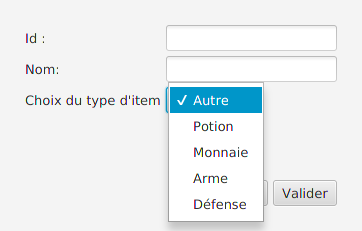
\includegraphics[width=4cm]{img/inclusItems.png}
	\end{figure}

	\section{Les compétences}
		Des compétences peuvent également être créer. Une prochaine mise à jour permettra de créer des compétences avec des actions influencant le joueur.
		\begin{figure}[H]
			\centering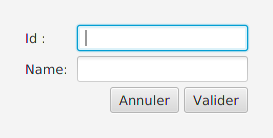
\includegraphics[width=4cm]{img/inclusSkills.png}
		\end{figure}

		Les compétences peuvent être apprise dès le début du livre (voir \ref{subsubsection:compétences}). Ils peuvent êgalement être demander en prérequis dans les liens (Voir \ref{chapter:lien}).
